\documentclass{beamer}
\usetheme{Warsaw}


\title[Working together]{Workflow and architecture patterns for working together 1: Workflows}
\author{Jacob Archambault}
\AtBeginSubsection[]
{
	\begin{frame}<beamer>{Outline}
		\tableofcontents[currentsection, currentsubsection]
	\end{frame}
}

\begin{document}
	\begin{frame}[plain]
		\titlepage
	\end{frame}
	\begin{frame}{Outline}
		\tableofcontents[pausesections]
		% You might wish to add the option [pausesections]
	\end{frame}
	\section{Current challenges and their canonical solutions}
	\begin{frame}{Challenges}
		\begin{itemize}
			\item coordinating multiple teams working in the same repository 
			\item lack of direct collaboration, and occasionally trust, between development, operations, and testing 
			\item late integration of contributor code 
			\begin{itemize}
				\item feedback delays 
				\item merge conflict regressions 
				\item sunk costs fallacy risks 
			\end{itemize}
			\item coupling of all services at the database layer 
			\begin{itemize}
				\item high storage costs 
				\item single point of failure risk 
				\item risk of cross-project interference 
			\end{itemize}
		\end{itemize}
	\end{frame}
	\begin{frame}{Canonical solutions to these challenges}
		\begin{itemize}
			\item multiple teams $\rightarrow$ inverse Conway maneuver 
			\item collaboration $\rightarrow$ business stream-aligned teams over activity oriented teams 
			\item late integration $\rightarrow$ adopting a true continuous integration workflow 
			\item database coupling $\rightarrow$ Bezos API mandate/``Microservices'' 
			
			
		\end{itemize}
	\end{frame}
	
	\section{DevOps 201}
	\subsection{Communication}
	\begin{frame}{1967: Conway's law}
		\begin{quote}
			`Organizations which design systems [...] are constrained to produce designs which are copies of the communication structures of these organizations.' - Melvin Conway, `How do Committees Invent?' Datamation, 1967
		\end{quote}
	\end{frame}
	\begin{frame}{Conway's law: examples}
		\begin{itemize}
			\item `If you have four groups working on a compiler, you'll get a 4-pass compiler' - The New Hacker's Dictionary, 1996
			\item front-end [devs] business layer [backend devs] monolithic database [DBA team] 
			\item a web api controller [manager]  delegates most business logic to business classes [developers] which are part of the same in-memory process [team], while serving as a single entry-point for wider cross-network [cross-team] communication.
		\end{itemize}
	\end{frame}
	\begin{frame}{Conway's law: more examples}
		\begin{itemize}
			\item separate \texttt{.csproj} projects for tests written by QA 
			\item separate development and config repositories for the same transaction signifying low communication between development and operations 
			\item all business documentation in the same repository, separate from the repositories that the documentation is for 
		\end{itemize}
	\end{frame}
	\begin{frame}{Conway's law: corollaries}
		\begin{itemize}
			\item Conway's law can't be fought 
			\item Teams working in the same part of the same codebase at the same time are the same team 
			\begin{itemize}
				\item separate the codebases for improved velocity 
				\item join the teams for improved code sharing and communication (Inverse conway maneuver)  
				\item branching-based strategies for team management compromise between the above approaches without their benefits
			\end{itemize}
		\end{itemize}
	\end{frame}
	\begin{frame}{1975: The Mythical Man Month, Fred Brooks}
		
		\begin{itemize}
			\item number of direct communication paths for $n$ individuals= $n(n-1)/2$
		\end{itemize}
		\begin{center}
			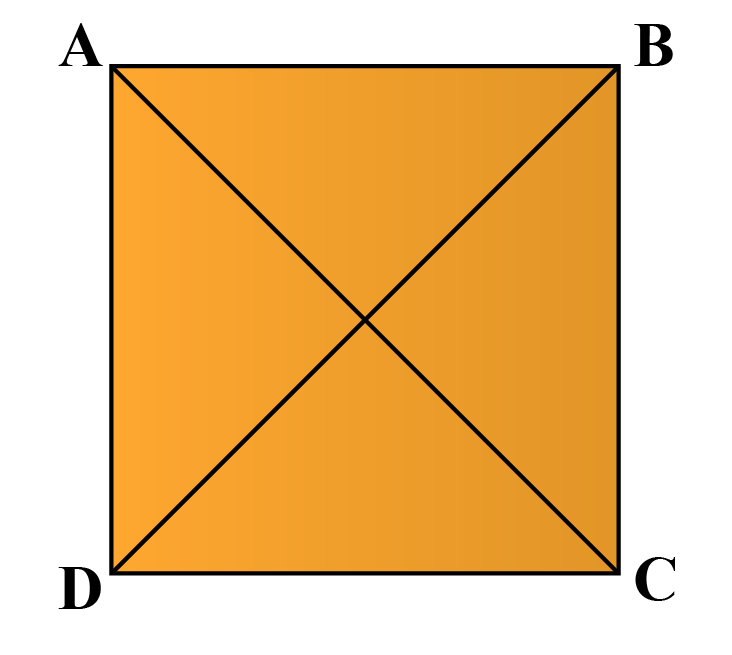
\includegraphics[width=.5\textwidth]{square}
		\end{center}
		
	\end{frame}
	\begin{frame}{1975: The Mythical Man Month, Fred Brooks}
		
		\begin{itemize}
			\item number of direct communication paths for $n$ individuals= $n(n-1)/2$
		\end{itemize}
		\begin{center}
			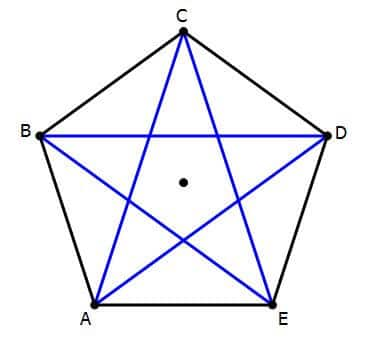
\includegraphics[width=.5\textwidth]{pentagon}
		\end{center}
		
	\end{frame}
	\begin{frame}{1975: The Mythical Man Month, Fred Brooks}
		
		\begin{itemize}
			\item number of direct communication paths for $n$ individuals= $n(n-1)/2$
		\end{itemize}
		\begin{center}
			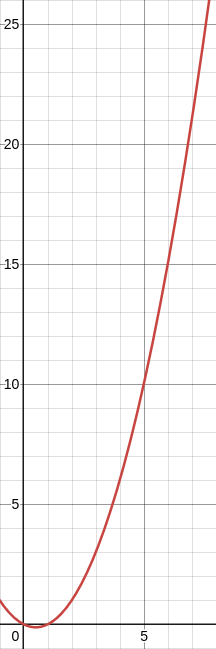
\includegraphics[width=.15\textwidth]{graph}
		\end{center}
	\end{frame}
	\begin{frame}{The Mythical Man Month, Fred Brooks (cont.)}
		\begin{itemize}
			\item corollary: adding more people to a project can lead not only to diminishing returns on delivery speed, but to objectively less work being completed
		\end{itemize}
		\begin{center}
			\begin{figure}
				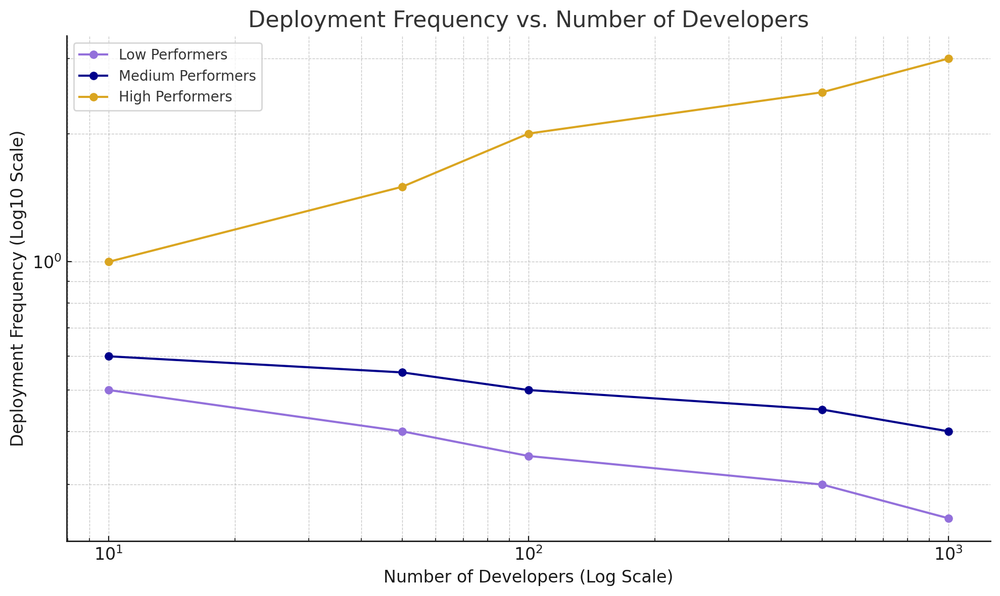
\includegraphics[width=.9\textwidth]{developers-deployments}
				%\caption*{Source: \url{https://devops-singularity.com/the-current-state-of-devops/}}
			\end{figure}
		\end{center}
	\end{frame}
	\subsection{Throughput}
	\begin{frame}{Just-in-time manufacturing and Goldratt's theory of constraints}
		\begin{itemize}
			\item Increase: throughput 
			\item Decrease: 
			\begin{itemize}
				\item operating costs 
				\item inventory 
				\item scrap 
			\end{itemize}
			\item Remove bottlenecks
		\end{itemize}
	\end{frame}
	\begin{frame}{Goldratt's theory of constraints (cont.)}
		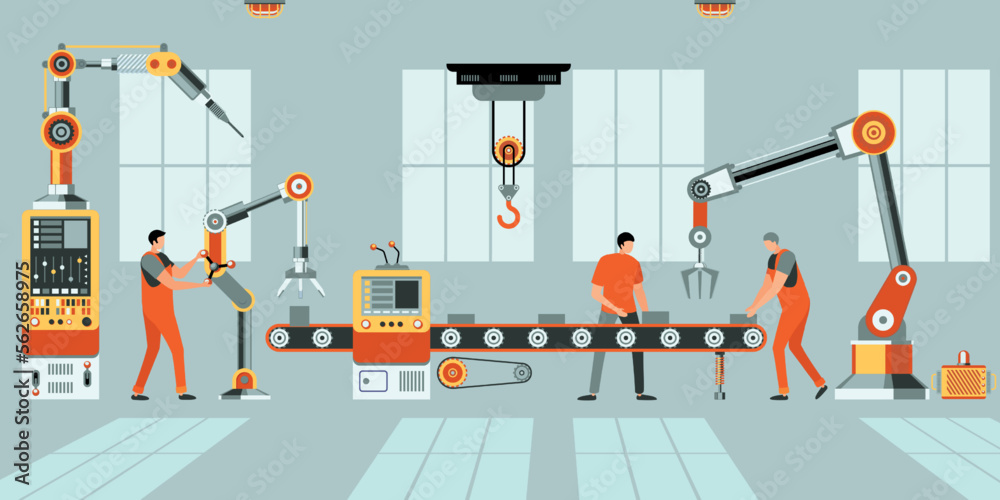
\includegraphics{assemblyline}
	\end{frame}
	\begin{frame}{2013: The State of DevOps Report}
		\begin{itemize}
			\item a series of surveys of over 36,000 professionals 
			\item Led by a PhD statistician, Nicole Forsgren, from 2013-2019 
			\item Uses \emph{cluster analysis} to discover groupings - has no prior understanding of what counts as good or bad.
		\end{itemize}
	\end{frame}
	\begin{frame}{The State of DevOps Report: throughput metrics}
		\begin{itemize}
			\item lead time for changes 
			\item deployment frequency 
		\end{itemize}
	\end{frame}
	\begin{frame}{The State of DevOps Report: stability metrics}
		\begin{itemize}
			\item change failure rate 
			\item mean time to restore
		\end{itemize}
	\end{frame}
	\begin{frame}{The State of DevOps Report: results}
		\begin{quote}
			`Astonishingly, these results demonstrate that there is no trade-off between improving performance and achieving higher levels of stability and quality. Rather, high performers do better at all of these measures. This is precisely what the Agile and Lean movements predict, but much dogma in our industry still rests on the false assumption that moving faster means \emph{trading off} against other performance goals, rather than enabling and reinforcing them.'  - Nicole Forsgren, Jez Humble, and Gene Kim, \emph{Accelerate} (2017), p. 14
		\end{quote}
	\end{frame}
	\begin{frame}{The State of DevOps Report: results}
		\rightline{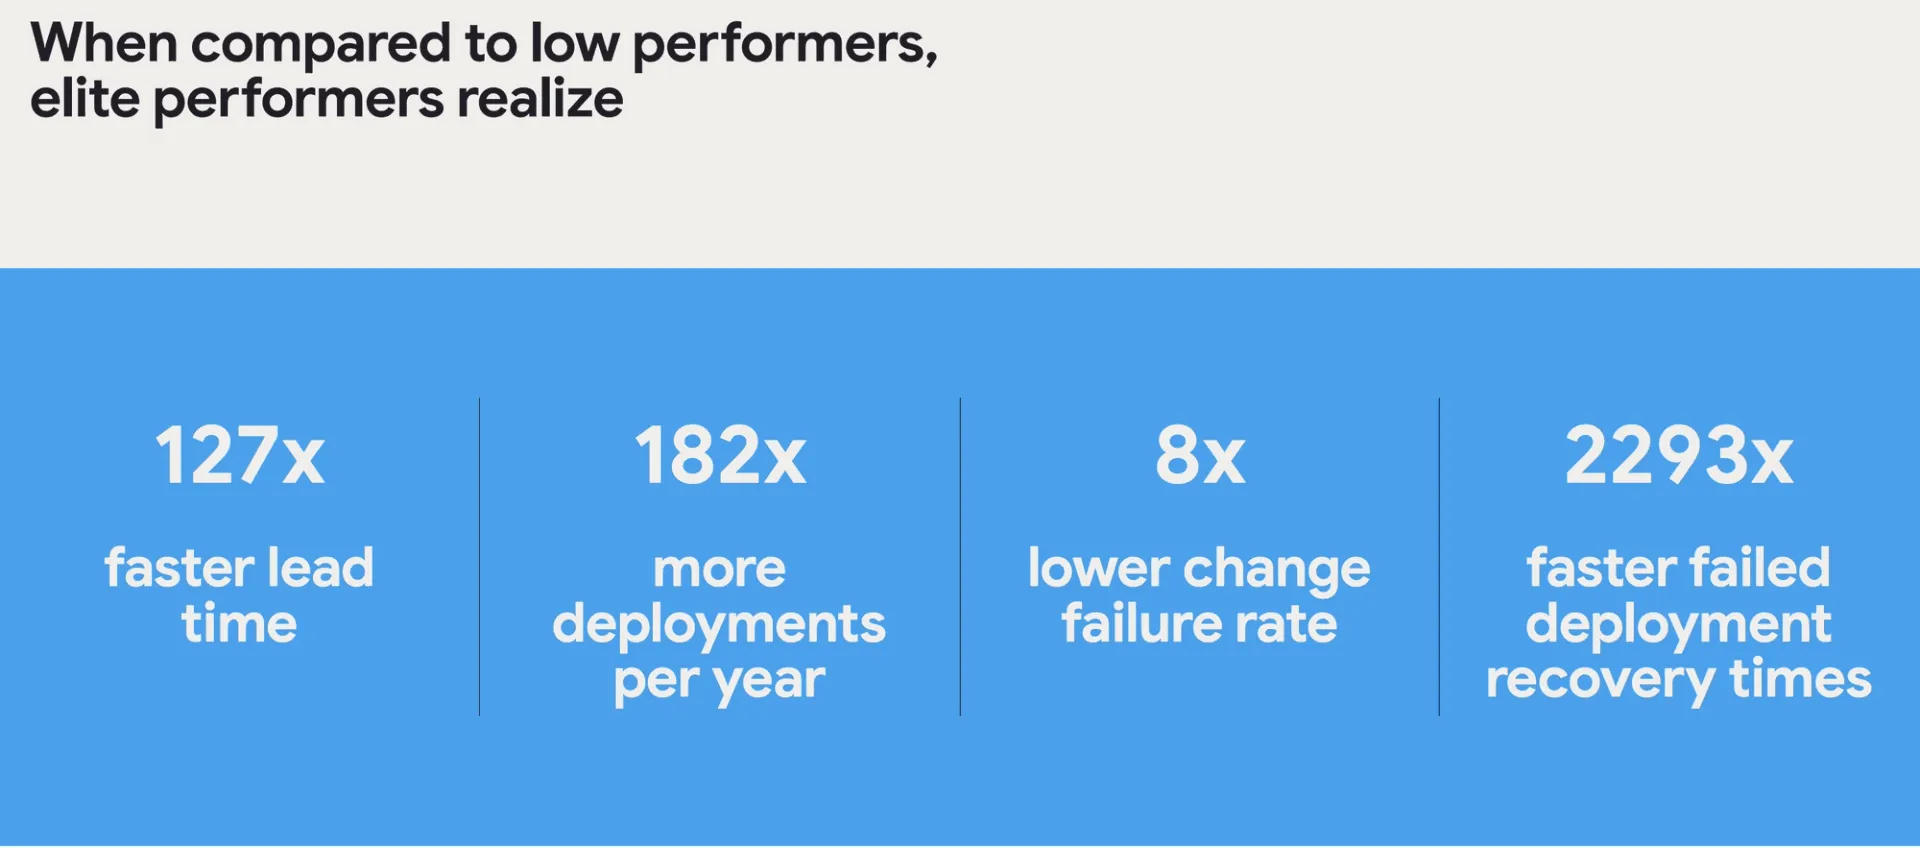
\includegraphics[width=1\textwidth]{dora2024}}
		
		\rightline{- 2024 State of DevOps Report}
	\end{frame}
	\section{Branching and continuous integration}
	\subsection{Definition}
	\begin{frame}{Defining continuous integration}
		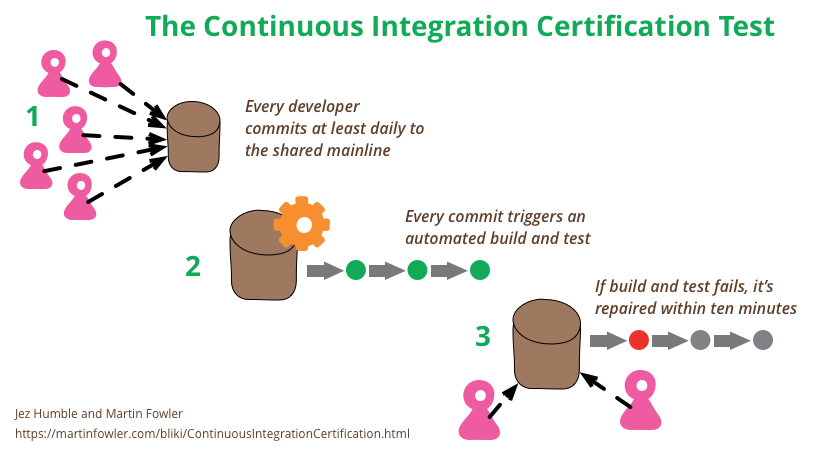
\includegraphics[width=1\textwidth]{cicert}
	\end{frame}
	\subsection{CI Branching patterns}
	\begin{frame}{Continuous integration branching patterns}
		\begin{itemize}
			\item  don't 
			\item as little as possible, for as short a time as possible, at least daily 
		\end{itemize}
	\end{frame}
	\subsection{Trade-offs}
	\begin{frame}{Continuous integration: trade-offs}
		\begin{quote}
			Continuous Integration applies a different trigger for integration - you integrate whenever you've made a hunk of progress on the feature and your branch is still healthy. There's no expectation that the feature be complete, just that there's been a worthwhile amount of changes to the codebase. The rule of thumb is that “everyone commits to the mainline every day”, or more precisely: you should never have more than a day's work sitting unintegrated in your local repository. 
			
			\rightline{- Martin Fowler, ``Branching Patterns''}
		\end{quote}
	\end{frame}
	\begin{frame}
		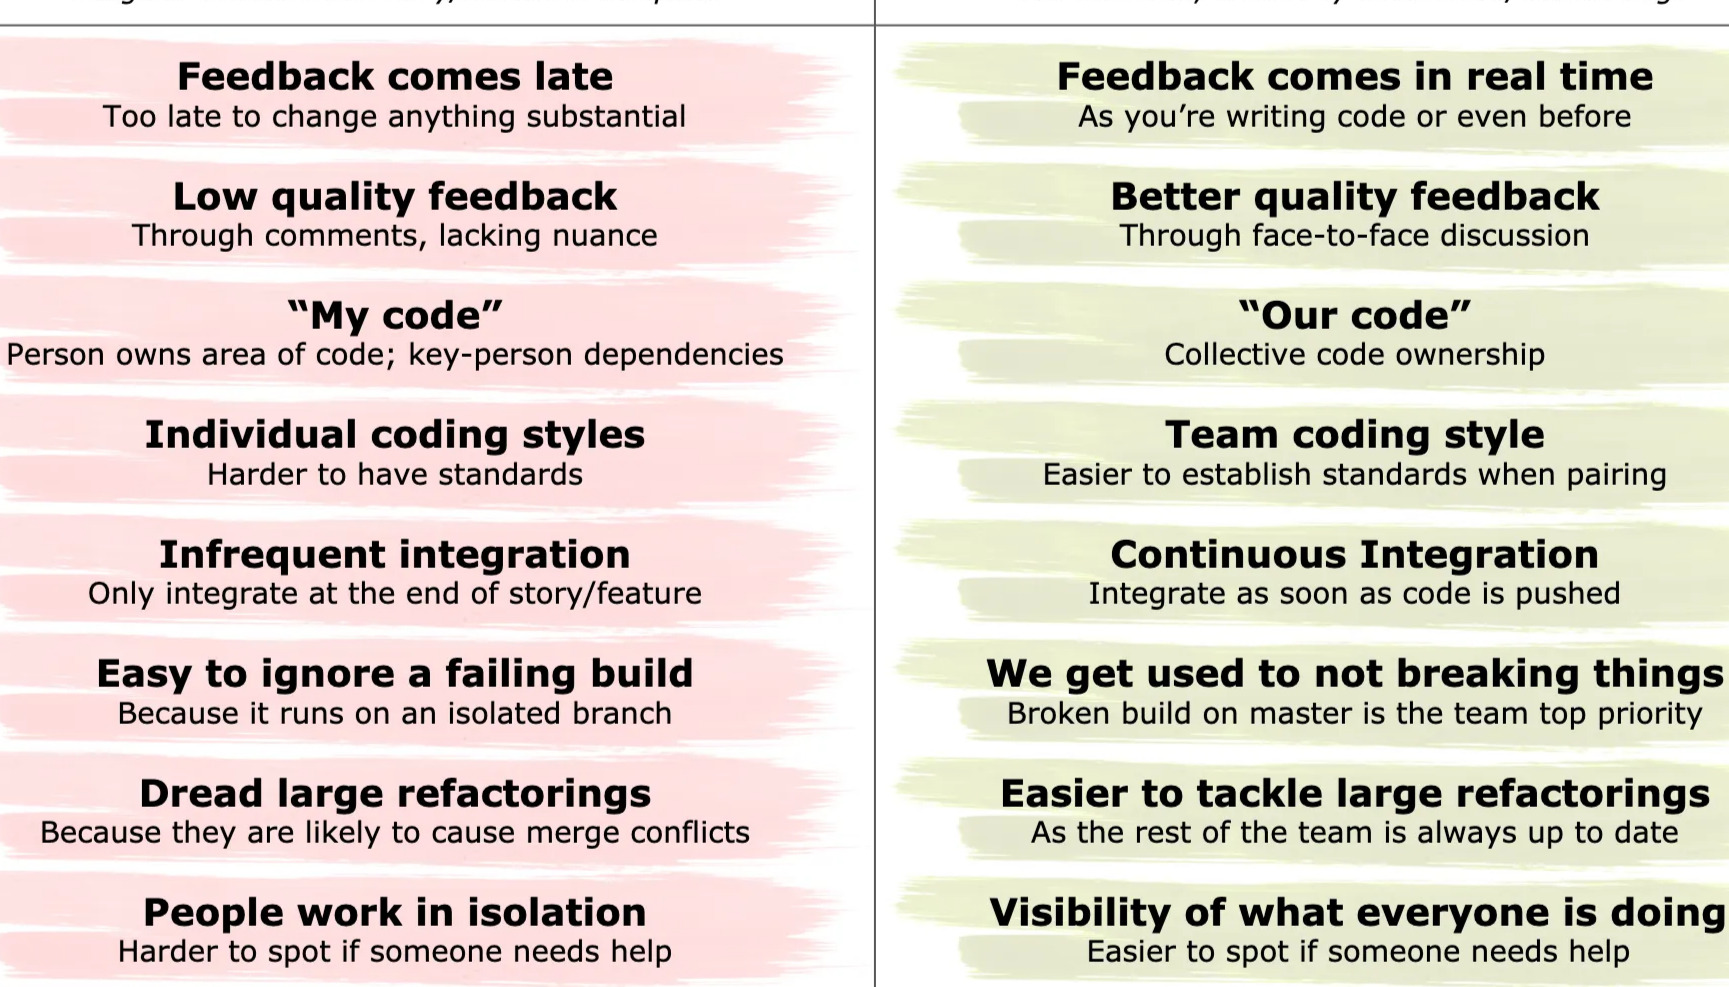
\includegraphics[width=1\textwidth]{tbd}
	\end{frame}
	\subsection{Enablers}	
	\begin{frame}{Continuous integration: Enablers}
		\begin{itemize}
			\item fast PR turnaround 
			\item improving CI pipeline runtime 
			\item team discipline 
		\end{itemize}
	\end{frame}
	\subsection{Benefits}
	\begin{frame}{Continuous integration: benefits}
		\begin{itemize}
			\item High performers have the shortest integration times and branch
			lifetimes, with branch life and integration typically lasting hours. 
			\item Low performers have the longest integration times and branch 
			lifetimes, with branch life and integration typically lasting days. 
			\item These differences are statistically significant
			
			\rightline{- 2017 State of DevOps Report, p. 41}
		\end{itemize}
	\end{frame}
	\begin{frame}{Continuous integration, benefits (cont.)}
		\begin{quote}
			Taken together, continuous delivery and organizational culture explain 28.8\% of the variance in IT
			performance. 
			
			- Forsgren and Humble (2016), `The Role of Continuous Delivery in IT and Organizational Performance
		\end{quote}
	\end{frame}
	\begin{frame}{Continuous integration, benefits (cont.)}
		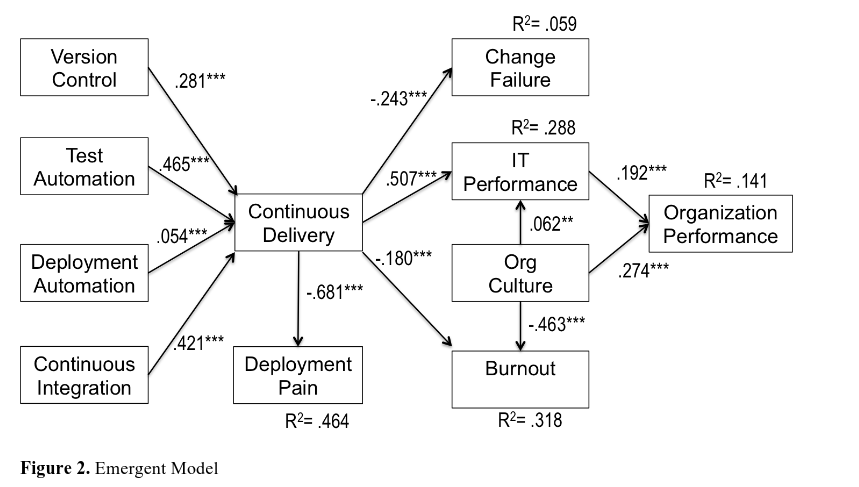
\includegraphics[width=1\textwidth]{CIbenefits}
	\end{frame}
	
	\section{Communication and throughput anti-patterns and solutions}
	\subsection{Communication anti-pattern: local optimization}
	\begin{frame}{communication anti-pattern: local optimization}
		\begin{itemize}
			\item example: separate (DevOps, QA, operations, support) team 
			\item leads to bottlenecks 
			\item delays communication 
			\item discourages cross-functional collaboration 
			\item punishes untracked work (e.g. thorough code reviews/dev testing, helping blocked colleagues)
		\end{itemize}
	\end{frame}
	\begin{frame}{Solution}
		\begin{itemize}
			\item autonomous, cross-functional teams with `t-shaped' employees 
			\item communities of practice 
		\end{itemize}
	\end{frame}
	\begin{frame}{Revisiting Conway's law: defining a team}
		\begin{itemize}
			\item A \textit{team} is the minimal socio-technical unit that can deliver a production change with no additional coordination beyond mandated governance or custodial controls. 
			\begin{itemize}
				\item pull requests 
				\item testing 
				\item deployment 
			\end{itemize}
		\end{itemize}
	\end{frame}
	\subsection{Throughput anti-pattern: Gandalf vs. the Balrog}
	\begin{frame}{Throughput anti-pattern: Gandalf vs. the Balrog}
		\begin{center}
			
\includegraphics[width=.5\textwidth]{gandalf-balrog}
		\end{center}
	\end{frame}
	\begin{frame}{Throughput anti-pattern: Gandalf vs. the Balrog}
		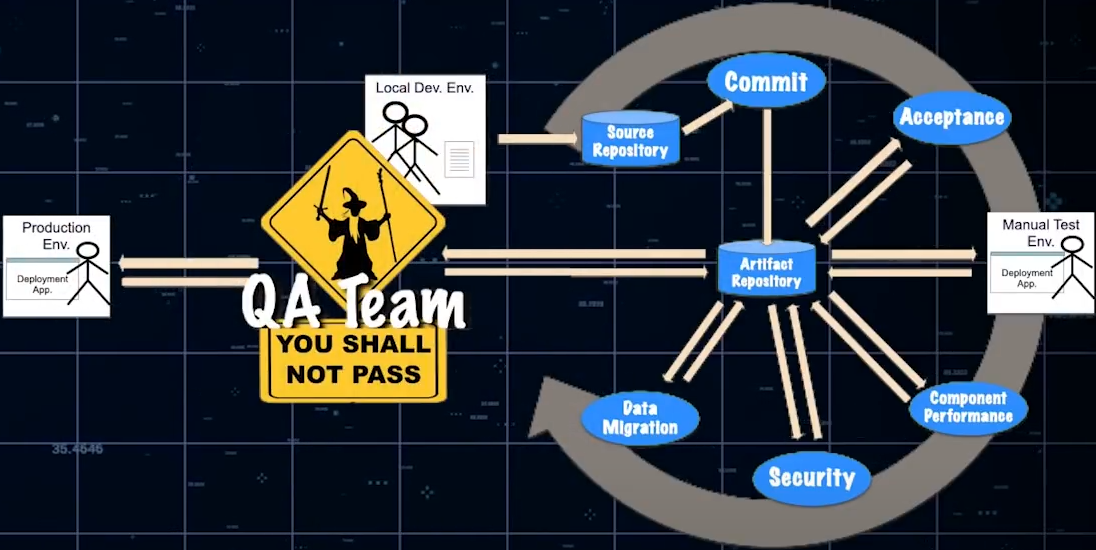
\includegraphics[width=\textwidth]{gandalf}
	\end{frame}
	\begin{frame}{Throughput anti-pattern: Gandalf vs. the Balrog}
		\begin{itemize}
			\item change approval boards  
			\item pre-merge code reviews  
			\item `bridge-to-nowhere' pipelines 
			\item these all increase lead time
		\end{itemize}
	\end{frame}
	\begin{frame}{Throughput anti-pattern solutions: aggressively parallelize work}
		\begin{itemize}
			\item pair programming  
			\item parallelized pipeline builds for `wide' pipelines 
			\item one build artifact for all pipeline stages 
			\item share responsibility
		\end{itemize}
	\end{frame}
	\begin{frame}{Defining throughput for our project}
		\begin{itemize}
			\item Avoid `thrashing' metrics 
			\item \textit{Throughput} - the total lapsed time from local commit to production deployment 
			\item \textit{Throughput*} - the total lapsed time from local commit to user acceptance testing handoff 
		\end{itemize}
	\end{frame}
	\section{Conclusion}
	\begin{frame}{Conclusion}
		\begin{itemize}
			\item Reduce goal misalignment 
			\item stop people from waiting on each other  
			\item work in small batches 
			\item That's mostly it
			
		\end{itemize}
	\end{frame}
	\begin{frame}[plain]
		\titlepage
	\end{frame}
\end{document}
